\section{Model}
\subsection{Sections}
Memories are organized so that each output data pin \texttt{DQ} is interleaved with \texttt{VDDQ} and \texttt{VSSQ} power pins as in \autoref{fig:pin-layout} to help the receiver in recognizing the data which may be distorted at such high speeds.
\begin{figure}[htbp]
	\center
	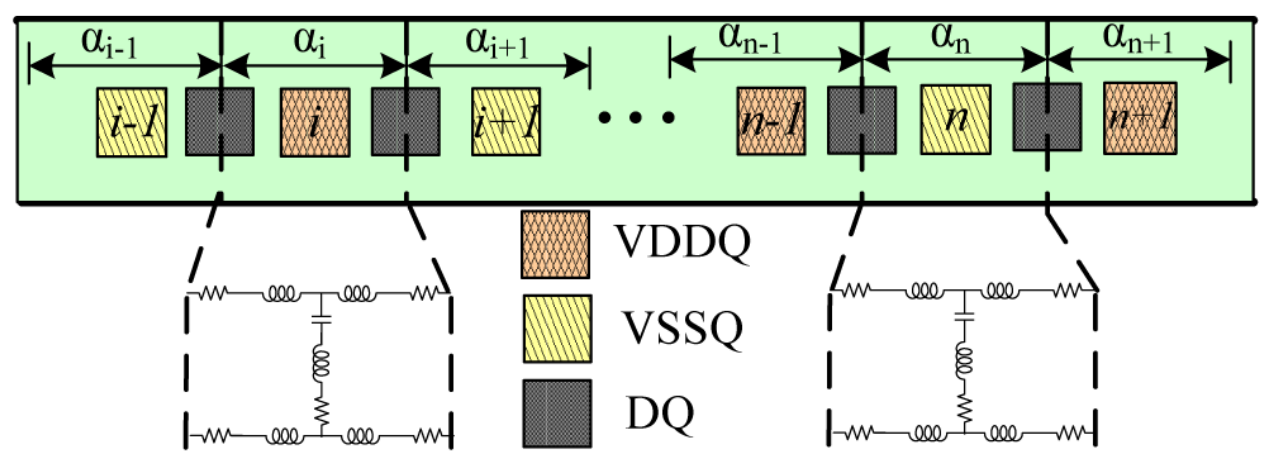
\includegraphics[width = \textwidth]{img/pin-layout}
	\caption{Pin layout of a memory chip}
	\label{fig:pin-layout}
\end{figure}

It is possible to split the power bus in sections - one for each power pin - of lengths $\alpha_i$ as shown in \autoref{fig:pin-layout}. Each section can be modeled with a two port device strucured as in \autoref{fig:tsection-model}.
\begin{figure}[htbp]
	\center
	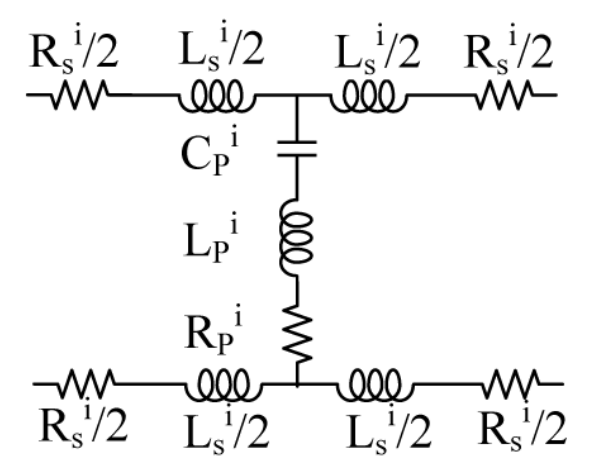
\includegraphics[width = 0.4\textwidth]{img/tsection-model}
	\caption{Model of a single section of a memory output}
	\label{fig:tsection-model}
\end{figure}

\subsection{Parameters}
\label{ssec:parameters}
Each section has five characterizing parameters: $R^i_s$, $L^i_s$, $R^i_p$, $L^i_p$, $C^i_p$ which depend on the overall Per-Unit-Length (PUL) parameters $R_s$, $L_s$, $R_p$, $L_p$, $C_p$ and the section length $\alpha_i$. PUL parameters also take the skin effect into consideration by using a DC resistance and an AC resistance which depends on frequency. The effective resistance of a memory section will be the greatest of the two for a given frequency.

In general, section parameters are computed from PUL parameters with the following formulas:
\begin{align*}
    R^i_s &= \alpha_i \max\left(R_{s,\,dc},\, R_{s,\,ac}\sqrt{\omega}\right) \\
    L^i_s &= \alpha_i L_s \\
    R^i_p &= \frac{1}{\alpha_i} \max\left(R_{p,\,dc},\, R_{p,\,ac}\sqrt{\omega}\right) \\
    L^i_p &= \frac{1}{\alpha_i} L_p \\
    C^i_p &= \alpha_i C_p
\end{align*}
Thanks to these formulas, it is possible to accurately represent the behavior of a power pin based on the power bus PUL parameters and the section lengths.

\subsection{Fitting}
\label{ssec:fitting}
While section lengths are known a-priori from layout information, PUL parameters can instead be determined by fitting real world electrical measurements. The measured quantity is the two port $Z$ matrix between two arbitrary power pins. In order to compare the model to its real world counterpart, the procedure in \autoref{ssec:from-parameters-to-Z-matrix} explains how the $Z$ matrix can be computed from the model parameters.

The fitting process is thus reduced to a multi-variable optimization process, where the unknowns are the PUL parameters and the error to the real world device is to be minimized. The error function $U\left(\vec{p}\right)$ can be expressed as:
\begin{align*}
    U\left(\vec{p}\right) &= \sum_{i = 0}^N \left|| Z_s\left(\vec{p}, f_i\right) - Z_m(f_i) |\right| ^2
\end{align*}
where $\vec{p}$ is a vector representing the device PUL parameters, $N$ is the total number of measured frequencies, $f_i$ is the i-th measured frequency, $Z_s$ is the impedance matrix obtained from the simulation and $Z_m$ is the measured matrix.

\subsection{From PUL Parameters to Z Matrix}
\label{ssec:from-parameters-to-Z-matrix}
In order to obtain $U(\vec{p})$ it is necessary to compute $Z_s\left(\vec{p}, f_i\right)$, which means computing an impedance matrix starting from the model's PUL parameters.
\begin{enumerate}
    \item Compute each section's parameters from PUL parameters as in \autoref{ssec:parameters}
    \item Compute each section's ABCD matrix with
    \begin{equation*}
        \text{ABCD} = \begin{bmatrix}
            1 + z_i y_i   & (z_i y_i + 2) z_i \\
            y_i           & 1 + z_i y_i
        \end{bmatrix}
    \end{equation*}
    where
    \begin{align*}
        z_i &= j \omega L_s^i + R_s^i \\
        y_i &= \frac{j \omega C_p^i}{1 + j\omega R_p^i C_p^i - \omega^2 L_p^i C_p^i}
    \end{align*}
    \item Divide the layout into three groups by cumulating ABCD matrices: before port 1 ($M_1 = \prod_{i = 0} ^ \text{P1} \text{ABCD}_i$), between port 1 and port 2 ($M_2 = \prod_{i = \text{P1}} ^ \text{P2} \text{ABCD}_i$) and after port 2 ($M_1 = \prod_{i = \text{P2}} ^ R \text{ABCD}_i$).

    \item Compute the $Y$ matrix with
    \begin{align*}
        Y(1, 1) &= \frac{M_1(2, 1)}{M_1(2, 2)} + \frac{M_2(2, 2)}{M_2(1, 2)} \\
        Y(1, 2) &= -\frac{1}{M_2(1, 2)} \\
        Y(2, 1) &= Y(1, 2) \\
        Y(2, 2) &= \frac{M_2(1, 1)}{M_2(1, 2)} + \frac{M_3(2, 1)}{M_3(1, 1)}
    \end{align*}
    \item Invert $Y$ to get the desired $Z$ matrix
\end{enumerate}

\subsection{Results}
After finding the best $\vec{p}$ that minimizes $U(\vec{p})$, the resulting PUL parameters are a good description of the physical device which limits the model error. The simulation ran from the author returns the results shown in \autoref{fig:zmatrix-paper}, which show how close the simulation is to the actual measurements.

\begin{figure}[htbp]
    \center
    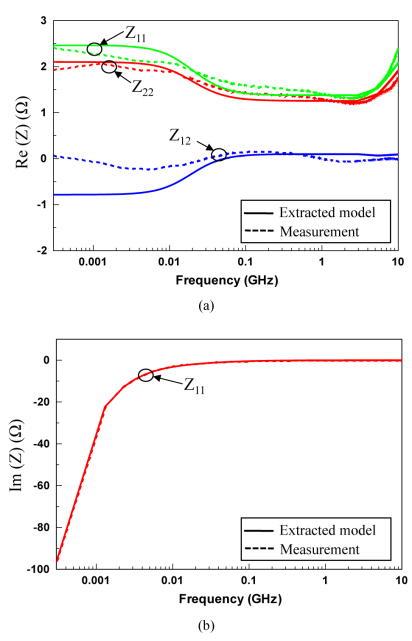
\includegraphics[width = 0.4\textwidth]{img/zmatrix-paper}
    \caption{Results from paper}
    \end{figure}
    \label{fig:zmatrix-paper}
